\documentclass[a4paper,12pt]{scrartcl}
\usepackage{setspace}
\usepackage[utf8x]{inputenc}
\usepackage{ngerman}
\usepackage{graphicx}
\usepackage{enumerate}
\usepackage{float}
\usepackage[font=small,labelfont=bf,singlelinecheck=false]{caption}
\usepackage[headsepline,plainheadsepline]{scrpage2}
\pagestyle{scrheadings}
\ohead[]{Christian Casar, Maximilian Menzel}
\ihead{HR - Blatt 4}



\begin{document}
\parindent0mm
\restylefloat{figure}
\setcapindent{0pt}
\subsubsection*{Parallelisierung mit OpenMP}
Wie in Tabelle 1 zu sehen wurde mit den vorgenommenen Änderungen am Quelltext ein Speedup um den Faktor neun erreicht. Mit einer höheren Iterationszahl hätte dieser Wert sich wahrscheinlich noch ein wenig höher schrauben lassen.
\begin{table}[!h]
\begin{tabular}{|l|r|r|r|r|}
\hline
Implementation&1. Messung&2. Messung&3. Messung&Mittel\\
\hline
sequentiell&	1146,8643&	1146,7031&	1146,5567&	1146,7080\\
\hline
OpenMP	&137,0301	&122,0230	&121,7702&	126,9411\\
\hline
\end{tabular}
\caption{\textbf{Laufzeitmessung der verschiedenen Implementationen.}\\ 12 Threads, 512 Interlines, 1024 Iterationen, Messwerte jeweils in Sekunden}
\end{table}
\subsubsection*{Umsetzung der Datenaufteilung}
Die Umsetzung der Datenaufteilung wurde jeweils in einer eigenen \texttt{c-Datei} vorgenommen bzw. die zeilenweise Aufteilung in der ursprünglichen \texttt{partdiff-openmp.c}, da sie genau der ursprünglichen Aufteilung entspricht. Es wurden die in Tabelle 2 aufgeführten Aufrufparameter gewählt, um mit einer relativ großen Datenmenge (1024 Interlines) zu arbeiten.

Dabei hat sich gezeigt, dass die spaltenweise Aufteilung mit Abstand am langsamsten arbeitet. Diese Tatsache ist vermutlich wieder mit der hohen Anzahl cache-misses zu erklären. Durch die Parallelisierung können zwar mehr Daten gleichzeitig bearbeitet werden, jedoch müssen die nachfolgenden Spaltenelemente immer erst zusätzlich in den Cache geladen werden. Für den Fall, dass manche Threads schneller als andere arbeiten, könnte sich hier eventuell für benachbarte Spalten positive Effekte einstellen. Durch das zeilenweise Caching könnte für hinterherhinkende aus Datensicht benachbarte Threads bereits das benötigte Spaltenelement durch den schnelleren Thread vorgecached sein.

Der Geschwindigkeitsunterschied zwischen der element- und zeilenweise Aufteilung lässt sich vermutlich durch den erhöhten Verwaltungsaufwand bei der elementweise Aufteilung erklären. Da für jedes neue Element ein neuer Thread erstellt bzw. bei Wiederverwendung wohlmöglich reinitialisiert werden muss, verlangsamt dieser zusätliche Overhead die Werteberechnung, da mehr Zeit mit Datenzuteilung als Rechnen verbraucht wird. 

\begin{table}[!h]
\begin{tabular}{|l|r|r|r|r|r|}
\hline
Aufteilung&1. Messung&2. Messung&3. Messung&Mittel\\
\hline
Spalten	&462,5158	&462,0107	&469,3247	&464,6171\\
\hline
Zeilen	&265,1645	&264,5286	&263,9908	&264,5613\\
\hline
Elemente	&307,6507	&306,1153	&307,3371	&307,0344\\
\hline
\end{tabular}
\caption{\textbf{Laufzeitmesung der verschiedenen Datenaufteilungen.}\\ 12 Threads, 1024 Interlines, 512 Iterationen, Messwerte jeweils in Sekunden}
\end{table}

\subsubsection*{Vergleich der OpenMP-Scheduling-Algorithmen}
Zum Test der Scheduling-Algorithmen wurde die element- sowie spaltenweise Aufteilung verwendet. Für die elementweise Aufteilung stellt sich die statische Verteilung von je zwei Interationen den Testergebnisse nach am effizientesten heraus. Die starke Zeitzunahme für \textit{static, 4} lässt sich eventuell mit einer Lastspitze auf dem Cluster erklären, da für die nachfolgenden Messungen wieder eine deutliche Verbesserung in den Berechnungszeiten zu sehen ist. Auch im Vergleich zu der Leistungsmessung aus Aufgabe 2 lässt sich ein leichter Zugewinn bei der Ausführungszeit gegenüber dem default-Scheduling erkennen.

Für die spaltenweise Aufteilung stellt sich kein Algorithmus leistungsfähiger als ein anderer heraus. Auch hier wird die Laufzeit wahrscheinlich wieder hauptsächlich durch die hohe Anzahl an cache-misses beeinflusst.


\begin{table}[!h]
\begin{tabular}{|l|r|r|r|r|r|}
\hline
Aufteilung&1. Messung&2. Messung&3. Messung&Mittel\\
\hline
static, 1&	303,3490&	304,5333&	304,8386&	304,2403\\
\hline
static, 2	&274,9212	&277,7070	&298,0135	&283,5472\\
\hline
static, 4	&632,1384	&632,3892	&633,6942	&632,7406\\
\hline
static, 16	&321,0543	&321,5812	&323,5345	&322,0567\\
\hline
dynamic, 1	&318,6475	&320,6304	&321,2673	&320,1818\\
\hline
dyamic, 4	&321,1643	&322,1790	&322,5387	&321,9607\\
\hline
guided	&321,0404	&321,3633	&322,7657	&321,7231\\

\hline
\end{tabular}
\caption{\textbf{Laufzeitmessung der Scheduling-Algorithmen für \\elementeweise Datenaufteilung.} 12 Threads, 1024 Interlines, 512 \\Iterationen, Messwerte jeweils in Sekunden}
\end{table}

\begin{table}[!h]
\begin{tabular}{|l|r|r|r|r|r|}
\hline
Aufteilung&1. Messung&2. Messung&3. Messung&Mittel\\
\hline
sta1s	&428,6237	&429,0607	&437,0074	&431,5639\\
\hline
static, 2	&426,8766	&429,3899	&437,9806	&431,4157\\
\hline
static, 4	&423,6773	&428,2202	&440,3662	&430,7545\\
\hline
static, 16	&425,2349	&427,9638	&428,5170	&427,2386\\
\hline
dynamic, 1	&427,0579	&428,1837	&429,0229	&428,0882\\
\hline
dynamic, 4 	&426,8279	&429,4160	&442,7836	&433,0092\\
\hline
guided	&427,6589	&428,5139	&428,7597	&428,3108\\

\hline
\end{tabular}
\caption{\textbf{Laufzeitmessung der Scheduling-Algorithmen für \\spaltenweise Datenaufteilung.} 12 Threads, 1024 Interlines, 512 \\Iterationen, Messwerte jeweils in Sekunden}
\end{table}
\vspace{5cm}
\subsubsection*{Leistungsanalyse}
\textit{Wir haben die Messungen durchgeführt bevor es zu der Diskussion auf der Mailingliste kam. Der dritte Absatz der Aufgabenstellung wurde dabei so interpretiert, dass die \textquotedblleft schnellste Parallelisierung\textquotedblright die effizienteste sein soll also Messung 1 mit 12 Threads.}
\vspace{5mm}

\begin{table}[!h]
\begin{tabular}{|l|r|r|r|r|r|}
\hline
Threadzahl&1. Messung&2. Messung&3. Messung&Mittel\\
\hline
1	&1176,7816	&1177,8659	&1180,4819	&1178,3765\\
\hline
2	&622,4143	&622,7875	&623,1165	&622,7727\\
\hline
3	&428,8923	&429,3416	&429,4848	&429,2396\\
\hline
4	&331,0162	&332,8195	&333,5723	&332,4693\\
\hline
5	&271,2221	&271,2729	&271,8071	&271,4340\\
\hline
6	&225,9340	&227,2840	&227,3568	&226,8583\\
\hline
7	&195,8572	&196,1717	&196,7443	&196,2577\\
\hline
8	&172,6415	&172,7483	&173,0870	&172,8256\\
\hline
9	&156,2731	&156,2907	&156,2911	&156,2850\\
\hline
10	&143,1850	&142,8846	&143,0423	&143,0373\\
\hline
11	&146,1335	&130,5580	&130,7782	&135,8233\\
\hline
12	&122,0102	&121,6997	&121,5206	&121,7435\\

\hline
\end{tabular}
\caption{\textbf{Laufzeitmessung für verschiedene Threadzahlen.} \\512 Interlines, 1024 Iterationen, Messwerte jeweils in Sekunden}
\end{table}

Die Messungen wurden jeweils mit den in Tabelle 1 bzw. 2 angegebenen Parametern durchgeführt, wobei die Sinus-Störfunktion verwendet wurde. Für die Variation in der Threadzahl lässt sich wie in Abbildung 1 zu sehen eine starke Abnahme in der Laufzeit feststellen. Am Anfang skaliert die Leistung sehr gut mit der Zunahme an Threads bis im zweistelligen Threadbereich die Leistung sich nur noch geringfügig verbessert. 

Dies mag zu einem daran liegen, dass wir uns mit zunehmender Threadzahl der optimalen Laufzeit der openMP-Parallelisierung annähern, zusätzlich wird wohl auch der zunehmende Aufwand für die Threadverwaltung eine gewisse Rolle spielen.
\begin{figure}[!ht]
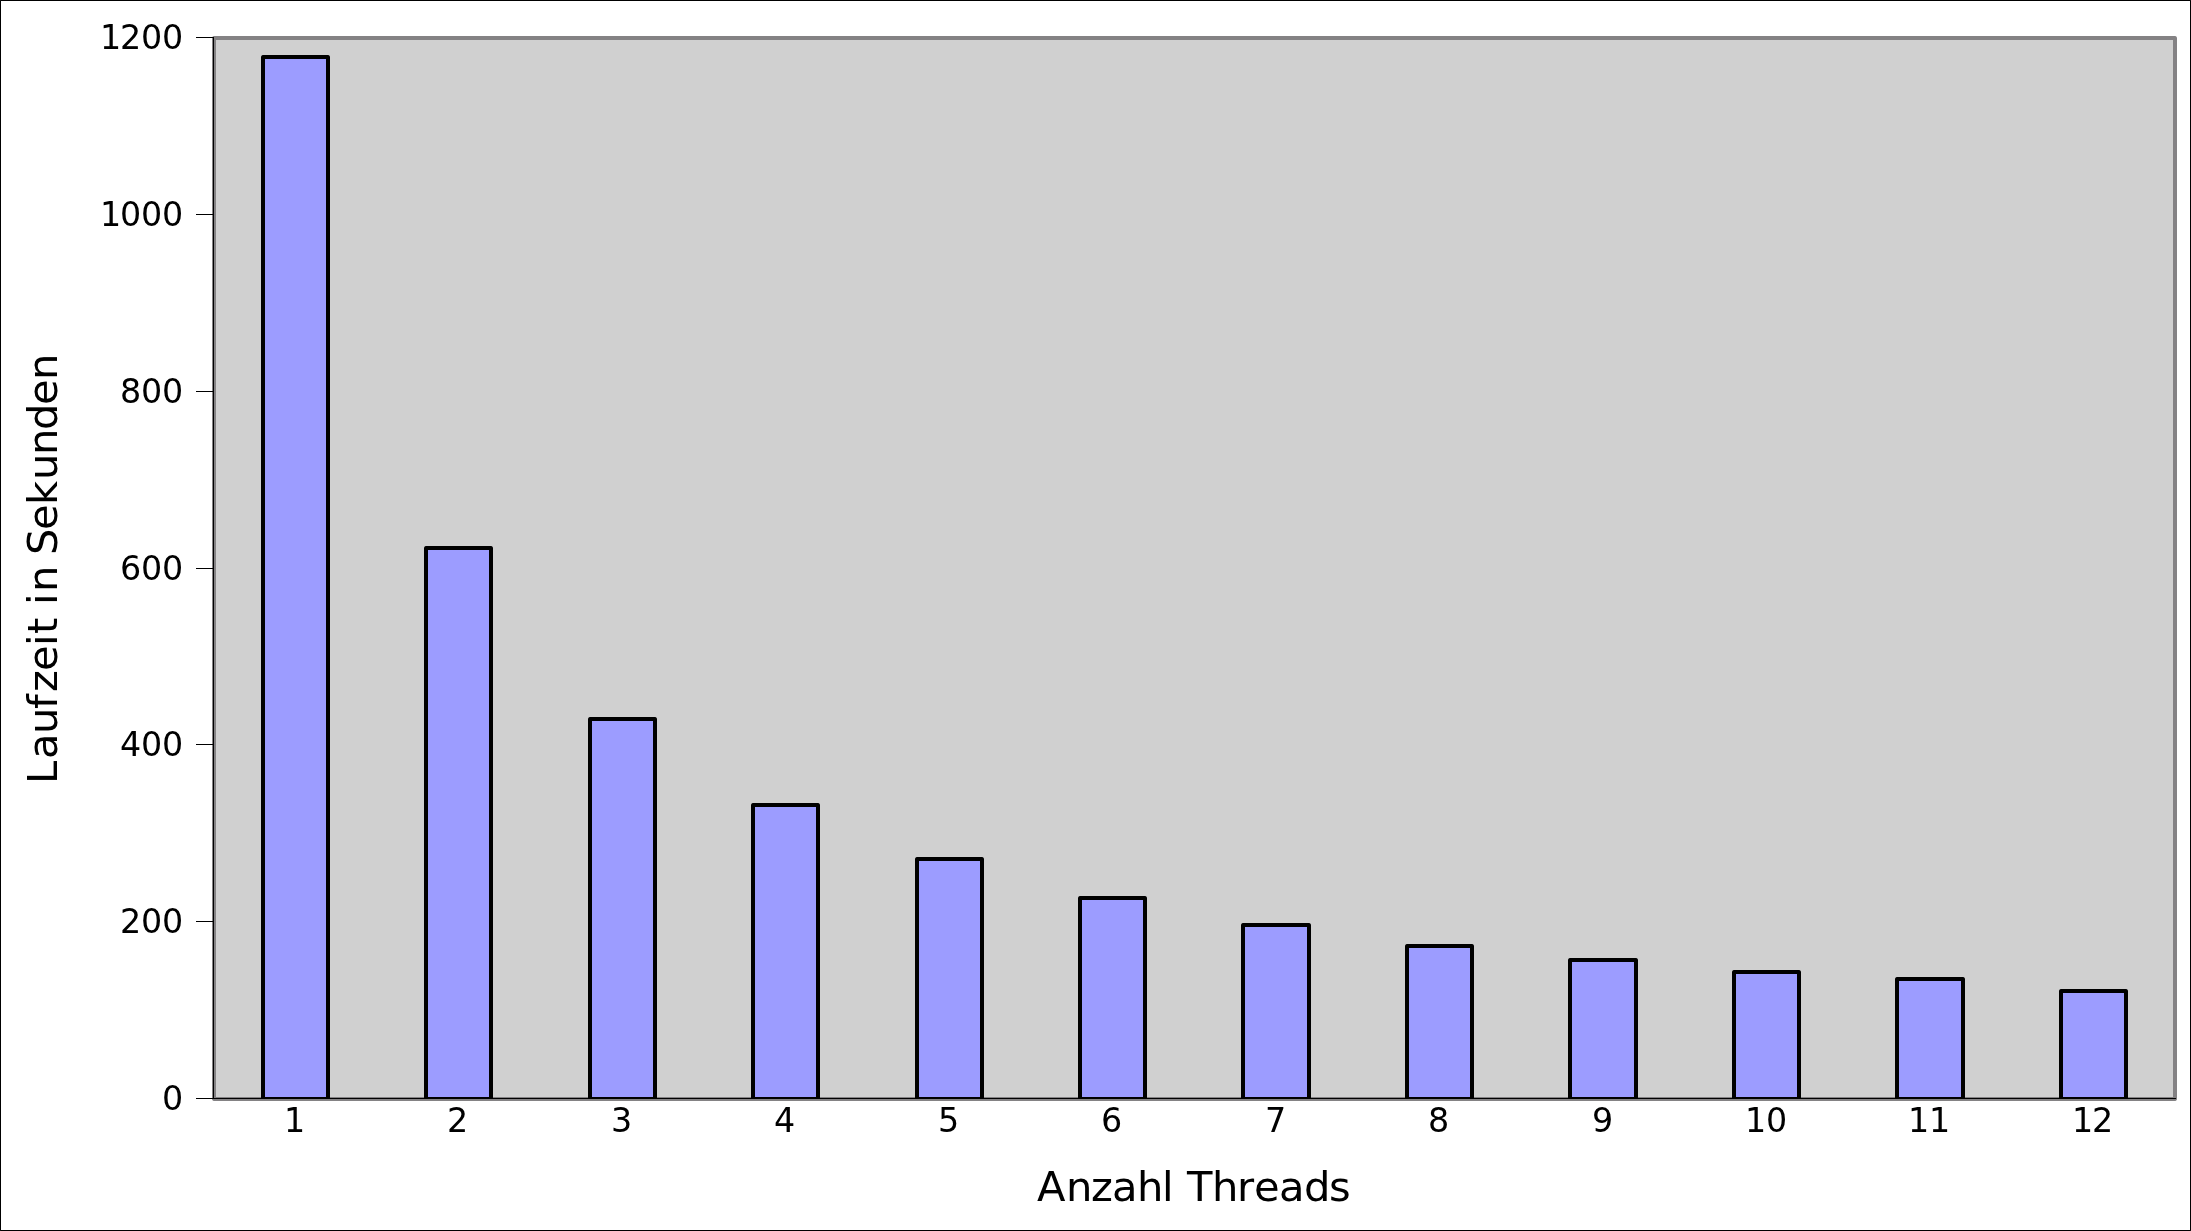
\includegraphics[width=14cm, height=8cm]{/home/christian/Uni/5_Semester/HR/HR-1213/Blatt4/leistungsgraph.png}
\caption{\textbf{Laufzeitmessung für verschiedene Threadzahlen.} \\512 Interlines, 1024 Iterationen}
\end{figure}



\begin{table}[!h]
\begin{tabular}{|l|r|r|r|r|r|}
\hline
Interlines&1. Messung&2. Messung&3. Messung&Mittel\\
\hline
1&	0,0084	&0,0079	&0,0092	&0,0085\\
\hline
2&	0,0120	&0,0124	&0,0115	&0,0120\\
\hline
4&	0,0197	&0,0184	&0,0203	&0,0194\\
\hline
8&	0,0673	&0,0450	&0,0553	&0,0559\\
\hline
16&	0,1353	&0,1673	&0,1755	&0,1594\\
\hline
32&	0,5009	&0,5733	&0,6675	&0,5806\\
\hline
64&	1,9164	&2,3005	&2,5123	&2,2430\\
\hline
128&	7,6345	&7,6356	&9,7240	&8,3314\\
\hline
256&	30,7198	&33,1656	&37,9655	&33,9503\\
\hline
512&	121,6844	&122,5537	&131,9247	&125,3876\\
\hline
1024&	486,2178	&488,4605	&545,6306	&506,7696\\

\hline
\end{tabular}
\caption{\textbf{Laufzeitmessung für verschiedene Interlinezahlen.} \\12 Threads, 1024 Iterationen}
\end{table}
 


\begin{figure}[H]
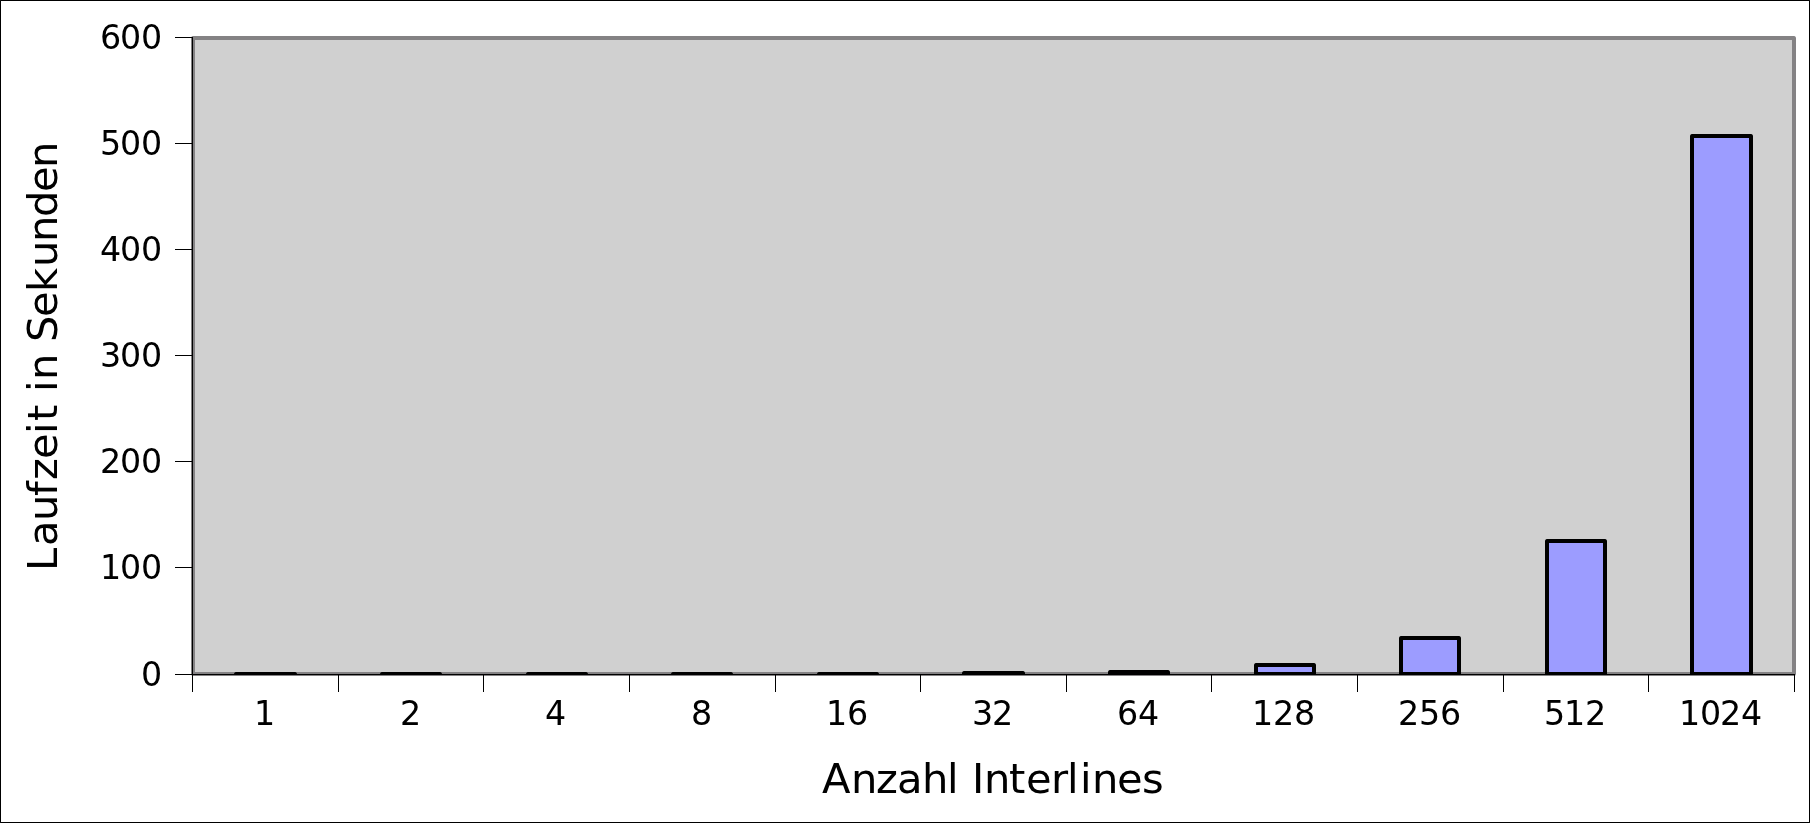
\includegraphics[width=14cm]{/home/christian/Uni/5_Semester/HR/HR-1213/Blatt4/leistungsgraph2.png}
\caption{\textbf{Laufzeitmessung für verschiedene Threadzahlen.} 12 Threads,\\ 1024 Iterationen, Messwerte jeweils in Sekunden}
\end{figure}
Für die Messwerte der variierenden Interlinezahlen lässt sich ebenfalls ein extrem starkes Wachstum feststellen. Wie in Abbildung 2 zu sehen, ist das Wachstum so stark, dass die Messwerte für geringe Interlinezahlen im Vergleich zu hohen Interlinezahlen verschwinden. Dieses Wachstum würde sich wohl jedoch auch bei einem nicht parallelisiertem Programm einstellen, da wir nichts am verwendeten Algorithmus verändert haben und dieser eine mindestens quadratische Laufzeit besitzt. Die Laufzeiten würde zwar sicherlich im Verhältnis stärker ansteigen und auch höhere Werte aufweisen, da die zur Verfügung stehenden Rechnerressourcen nicht effizient genutzt werden, aber die starke Laufzeitenzunahme liegt einfach an der zugrunde liegenden Problemstellung.
\end{document}
